\section{Method}
To address the data scarcity in 4D generative modeling, we first introduce \textbf{Rynn4DDataset 1.0} in Sec.~\ref{sec:data}, a large-scale hybrid dataset specifically curated for training feed-forward 4D generative models. Building upon this, Sec.~\ref{sec:generation} presents \textbf{\our}, a framework capable of co-generating future sequences—including RGB frames, depth maps, and optical flow from a single RGB-D observation and a linguistic task description. Finally, in Sec.~\ref{sec:action}, we introduce \textbf{\our-Policy}, which leverages the predictive 4D representations from \our to derive final robotic actions.


\subsection{Rynn4DDataset 1.0}
\label{sec:data}
To bridge the gap in large-scale 4D training data, we introduce Rynn4DDataset 1.0, a hybrid dataset comprising over 254.4 million video frames from human-centric (Epic-Kitchens~\citep{damen2020epic}, EgoVid~\citep{wang2024egovid}) and robotic manipulation datasets (RoboMIND~\citep{wu2024robomind}, RDT-1B~\citep{liu2024rdt}, Galaxea~\citep{jiang2025galaxea}, RoboCoin~\citep{wu2025robocoin}, AgiBot~\citep{bu2025agibot}).
Each frame is enriched with high-quality 4D pseudo-annotations: fine-grained instructions~\citep{bai2025qwen3}, monocular depth~\citep{lin2025depth}, and dense optical flow~\citep{morimitsu2025dpflow}. 
The statistics and composition of Rynn4DDataset 1.0 are visualized in Fig.~\ref{fig:data-dist}. 
The pipeline for our multimodal annotation is illustrated in Fig.~\ref{fig:data}.

\begin{figure}
  \centering
    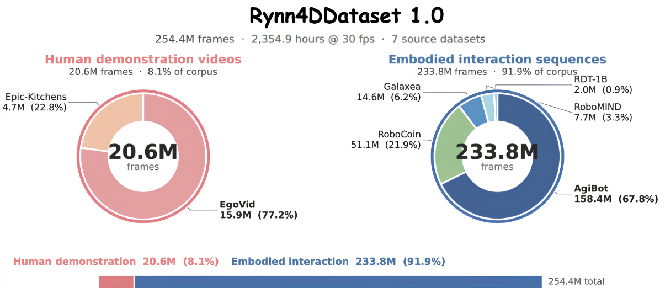
\includegraphics[width=0.85\linewidth]{Fig/data_dist.pdf}\\
  \caption{\textbf{Composition of the Rynn4DDataset 1.0 dataset.} We provide a large-scale hybrid collection of 254.4M frames, balancing human egocentric videos with diverse robotic manipulation data. This diversity ensures that the world model learns both general object interaction priors and robot-specific execution traces.}
  \label{fig:data-dist}
\end{figure}



\noindent 
\textbf{Video captioning.}
We use Qwen3-VL~\citep{bai2025qwen3} to generate captions for the video data~\citep{damen2020epic,wang2024egovid,wu2024robomind,liu2024rdt,jiang2025galaxea}. Specifically, we leverage the model's strong video-language understanding capabilities to produce detailed, structured descriptions of each video clip. The videos are first sampled at a frame rate of 1 FPS and split into segments of 5 seconds. For each segment, we provide the following prompt to the model:                                                                   

\begin{quote}                                                                                    \texttt{Please describe this video in detail. Include the following aspects:} \   

\texttt{1. The main subject and action in the video.} \ 

\texttt{2. The environment and background.} \       

\texttt{3. Any objects and their interactions.} \   

\texttt{4. The overall scene context and atmosphere.} \   

\texttt{Provide a concise but comprehensive caption in one paragraph.}                           \end{quote}                                                                                      

The generation is performed with a maximum output length of 512 tokens and a temperature of 0.7 to balance creativity and coherence. The generated captions are then collected and stored in JSON format for downstream tasks. 



\begin{figure}
  \centering
    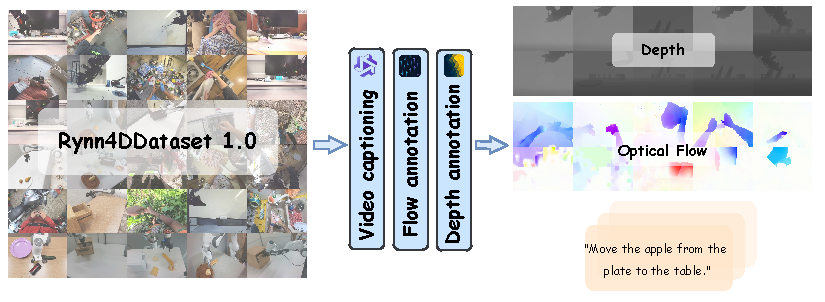
\includegraphics[width=\linewidth]{Fig/data.pdf}\\
  \caption{\textbf{Data Curation Pipeline.} The video data is collected from diverse sources and partitioned into short clips during data preprocessing. Each clip undergoes a multi-modal annotation process: (1) \textbf{Video Captioning}: Qwen3-VL~\citep{bai2025qwen3} generates
    detailed natural language descriptions of the video content; (2) \textbf{Optical Flow Estimation}: DPFlow~\citep{morimitsu2025dpflow} computes dense per-frame motion fields, which are visualized and saved as flow videos; (3) \textbf{Depth Estimation}: Depth Anything  
   3~\citep{lin2025depth} produces monocular depth predictions, which are upsampled to the original resolution and saved as depth videos with a global depth range of $[0.0, 5.0]$ meters.}
  \label{fig:data}
\end{figure}


\noindent 
\textbf{Optical flow annotation.}
We employ DPFlow~\citep{morimitsu2025dpflow}, a state-of-the-art optical flow estimation model. For each video, frame pairs are processed sequentially at native resolution, and the estimated flow fields are visualized via color encoding and saved as MP4 videos at 25 FPS.


\noindent 
\textbf{Depth annotation.}
We employ Depth Anything 3~\citep{lin2025depth}, specifically the \texttt{DA3NESTED-GIANT-LARGE-1.1} checkpoint, which provides dense per-frame depth predictions along with camera pose estimation. Each video is sampled at 30 FPS and processed at a working resolution of 392 pixels (short side, upper-bound resize).                                                                

To convert the estimated depth maps into viewable depth videos, we load the compressed depth arrays and upsample each frame to the original video resolution using bilinear interpolation. Depth values are clipped to a global range of $[0.0, 5.0]$ meters and quantized to 8-bit grayscale via $I = \lfloor d / d_{\max} \times 255 \rfloor$. The resulting frames are saved as RGB videos.



\subsection{3D Scene Reconstruction from Multi-Modal Videos}
\label{sec:3d_reconstruction}

A key advantage of the RGB-DF (\textit{i.e.}, RGB, depth, and optical flow) representation is its inherent geometric interpretability. By combining the co-generated depth and optical flow, we can reconstruct a temporally consistent 3D scene and derive \textit{metric scene flow}.

\noindent 
\textbf{Geometric Unprojection.}
Given the generated depth map $D_t$ at frame $t$, each pixel $\mathbf{p}_t = [u, v, 1]^\top$ in homogeneous coordinates is unprojected into the 3D camera space as:
\begin{equation}
    \mathbf{P}_t = D_t(u, v) \cdot \mathbf{K}^{-1} \mathbf{p}_t,
\end{equation}
where $\mathbf{K}$ is the camera intrinsic matrix. This process lifts the 2D projective sequence into a metric 3D point cloud $\mathcal{C}_t = \{\mathbf{P}_t^i\}_{i=1}^{H \times W}$.

\noindent 
\textbf{Metric Scene Flow Derivation.}
To capture the underlying 4D dynamics, we leverage the co-generated dense optical flow $\mathbf{f}_{opt} = [\Delta u, \Delta v]^\top$ to establish temporal correspondences. A 3D point $\mathbf{P}_t$ is tracked to its position at $t+1$ by:
\begin{equation}
    \mathbf{P}_{t+1} = D_{t+1}(u+\Delta u, v+\Delta v) \cdot \mathbf{K}^{-1} (\mathbf{p}_t + [\Delta u, \Delta v, 0]^\top).
\end{equation}
The \textit{3D scene flow} is then defined as $\mathbf{f}_{3D} = \mathbf{P}_{t+1} - \mathbf{P}_t$, representing the per-point metric displacement. This explicit 4D mapping ensures that the generated trajectories are not merely visual hallucinations but correspond to physically plausible 3D movements.

\noindent 
\textbf{Refinement and Visualization.}
To suppress artifacts at depth discontinuities, we apply a depth-gradient-based edge filter, masking out pixels where $\|\nabla D\| > \tau$. The resulting refined 3D trajectories are projected into a canonical bird's-eye view (BEV). In our qualitative analysis (see the ``3D Flow'' panel in Fig.~\ref{fig:teasor}), these trajectories are rendered as colored trails over a depth-ordered point cloud backdrop, providing an intuitive verification of the model's spatial-temporal coherence.

\begin{figure}[t]
  \centering
    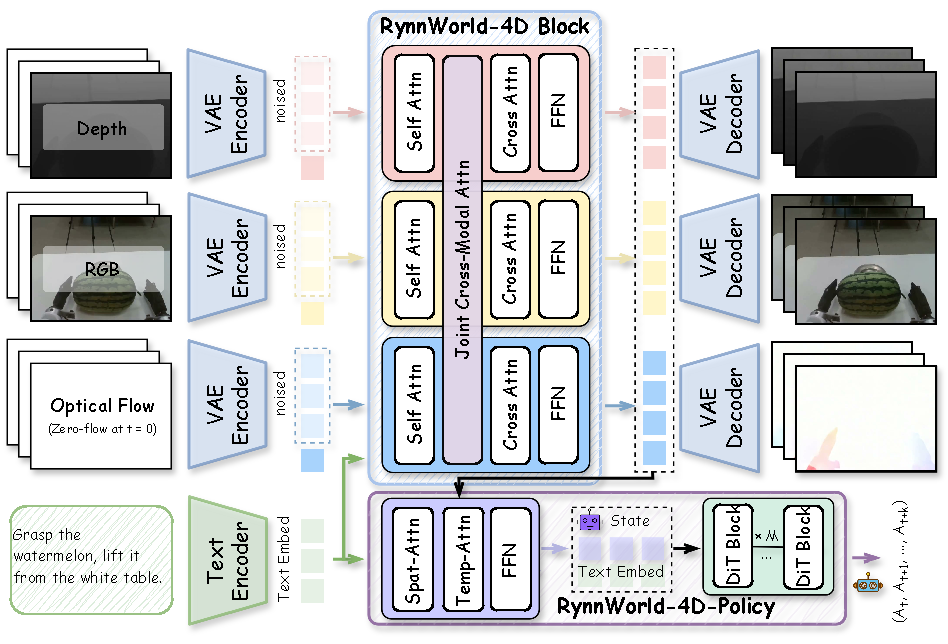
\includegraphics[width=\linewidth]{Fig/pipeline.pdf}\\
  \caption{\textbf{Overview of \our.} Our pipeline leverages the large-scale Rynn4DDataset 1.0 dataset to train a generative model capable of predicting future 4D sequences. Given a single RGB-D observation and a language instruction, \our co-generates future RGB frames, depth maps, and optical flow. These predictive 4D representations are then aggregated by \our-Policy to derive the final robot actions.}
  \label{fig:pipeline}
\end{figure}


\subsection{\our}
\label{sec:generation}
To achieve synchronized generation of RGB-DF sequences, we extend a pretrained video generative model into a tri-branch architecture (see the overview in Fig.~\ref{fig:pipeline}). This representation is not merely a concatenation of channels; it admits a physically-grounded unprojection into 3D scene flow, as detailed in Sec.~\ref{sec:3d_reconstruction}.
We denote the latents for modality $m \in \{\text{rgb, depth, flow}\}$ as $\bm{z}_t^m$, where $t \in [0, 1]$ represents the flow-matching timestep. Each $\bm{z}_t^m \in \mathbb{R}^{T \times C \times H \times W}$ encapsulates the entire temporal sequence of $T$ frames.

\noindent 
\textbf{Tri-branch Architecture.} 
To inherit the powerful generative priors of the pretrained model while capturing the distinct characteristics of each modality, we expand the single-branch backbone of Wan~\citep{wang2025wan} into a tri-branch structure. 
This decoupled design allows each modality to model its unique feature distributions, such as complex textures for RGB, spatial geometry for depth, and motion displacements for flow to mitigate representation interference among divergent modalities.


\noindent
\textbf{Joint Cross-Modal Attention.}
To enforce cross-modal consistency, we introduce a Joint Cross-Modal Attention (JA) module that is inserted every \emph{three} transformer blocks across all 30 Wan-2.2 layers (at layers $0, 3, 6, \dots, 27$), yielding 10 JA modules in total. Each JA module is appended after the intra-modal self-attention of its host block.

Before cross-modal mixing, each branch $m \in \{\text{rgb,depth,flow}\}$ receives a learnable modality embedding $\bm{e}^m \in \mathbb{R}^{1\times 1\times d}$ (zero-initialized so the module starts as a pure residual) and is normalized by a per-modality LayerNorm $\operatorname{LN}^{m}$ to align numerical scales across branches:
\begin{equation}
\tilde{\bm{z}}_l^m = \operatorname{LN}^{m}\bigl(\bm{z}_l^m + \bm{e}^m\bigr).
\end{equation}

Each branch $m$ produces \emph{one} query and \emph{one} shared key/value pair that is reused by all other branches' queries, reducing the parameter cost from $18d^2$ to $12d^2$ per block:
\begin{equation}
\bm{Q}_l^m = \operatorname{RMSNorm}_q\!\bigl(\operatorname{QProj}_l^m(\tilde{\bm{z}}_l^m)\bigr),\quad
[\bm{K}_l^m, \bm{V}_l^m] = \operatorname{KVProj}_l^m(\tilde{\bm{z}}_l^m),\quad
\bm{K}_l^m \!\leftarrow\! \operatorname{RMSNorm}_k(\bm{K}_l^m).
\end{equation}

Tokens are reshaped from $[B, T{\cdot}S, d]$ to $[B{\cdot}T, S, d]$ so that cross-modal attention is restricted to tokens of the \emph{same temporal frame} across modalities, and 3D Rotary Positional Embeddings are applied to $\bm{Q}_l^m$ and $\bm{K}_l^m$ to inject spatial position information consistently across branches. Each query attends only to the keys/values of the two complementary modalities:
\begin{equation}               
\bm{A}_l^m = \operatorname{Attn}\bigl(\operatorname{RoPE}(\bm{Q}_l^m),\;\operatorname{RoPE}(\bm{K}_l^{\text{cross}}),\;\bm{V}_l^{\text{cross}}\bigr),             \end{equation}
with $\bm{K}_l^{\text{cross}} = \operatorname{concat}(\{\bm{K}_l^j\}_{j\neq m})$ and $\bm{V}_l^{\text{cross}} = \operatorname{concat}(\{\bm{V}_l^j\}_{j\neq m})$.

Instead of the double zero-initialization used in ControlNet—which we found to introduce a saddle-point deadlock—we combine a \emph{zero-initialized} output projection $\operatorname{OutProj}_l^m$ with a learnable gate $g_l^m$ initialized to $1$:    
\begin{equation}
\hat{\bm{z}}_l^m = \bm{z}_l^m + \tanh(g_l^m)\cdot \operatorname{OutProj}_l^m(\bm{A}_l^m).                                \end{equation}                                                         

At initialization $\operatorname{OutProj}_l^m \equiv 0$ guarantees a smooth warm start from the Stage-1 checkpoint, while $\tanh(g_l^m) = \tanh(1) \neq 0$ ensures non-zero gradients flow into the gate so that it can decrease, increase, or change sign as training proceeds, preventing the joint pathway from being trapped at the origin. 


\noindent 
\textbf{Phased Training Strategy.} 
To bridge the significant distribution gaps between modalities, we propose a phased training paradigm: 
\textbf{Stage 1: Modality Adaptation.} In this initial stage, we disable the Joint Cross-Modal Attention and train the three branches independently. This allows the depth and flow branches to effectively adapt to their respective geometric and kinetic distributions. 
\textbf{Stage 2: Joint Attention Training.} We insert Joint Cross-Modal Attention modules every three layers across all 30 transformer blocks. The entire backbone and per-branch self-attention/FFN are frozen; only the Joint Cross-Modal Attention projections, RMSNorms, per-modality LayerNorms, tanh gates, and the three modality embeddings are trainable. Joint Cross-Modal Attention uses 3D RoPE and a frame-wise mask so cross-modal attention stays within the same temporal frame.
\textbf{Stage 3: Full-Parameter Joint SFT.} With the joint module already aligned, we unfreeze the entire model and continue on the full Rynn4DDataset 1.0.

\noindent
\textbf{Branch Dropout.}
In Stages 2 and 3, with probability $p_{\text{drop}}$ we randomly select one of $\{\text{depth}, \text{flow}\}$ at each training step and replace its noisy latent (frames $[1{:}]$) with pure Gaussian noise, forcing the JA modules to reconstruct it from the visible modalities. The RGB branch is never dropped, since it serves as the appearance anchor: destroying it would leave the joint module with no consistent reference.


\noindent
\textbf{Training Objective.}
All three stages are optimized using the flow matching objective~\citep{lipman2022flow}. For each modality $m \in \mathcal{M} = \{\text{rgb}, \text{depth}, \text{flow}\}$, we learn a velocity field $\bm{v}_\theta^m$ that transports Gaussian noise $\bm{\epsilon}^m$ to data $\bm{z}_0^m$ along the path $\bm{z}_t^m = (1-t)\bm{z}_0^m + t\bm{\epsilon}^m$. The first frame of each modality is the clean image-to-video conditioning latent (a real RGB frame, a real depth frame, and a zero-flow frame, respectively) and is excluded from supervision; we use the slice $[1{:}]$ to denote frames $1,\dots,T-1$. The total loss is:
\begin{equation}
\label{eq:flow_matching_main}
\mathcal{L}_{\text{total}} \;=\; \sum_{m \in \mathcal{M}} \lambda_m \,
        \mathbb{E}_{\bm{z}_0^m, \bm{\epsilon}^m, t, \bm{c}}
        \!\left[\bigl\| \bm{v}_\theta^m\!\bigl(\bm{z}_t^m, t, \bm{c}\bigr)_{[1{:}]}
        - \bigl(\bm{\epsilon}^m - \bm{z}_0^m\bigr)_{[1{:}]} \bigr\|_2^2\right],
\end{equation}                 
where $\bm{c}$ denotes the text prompt together with the initial RGB-D observation, and $\bm{\epsilon}^{\text{rgb}} = \bm{\epsilon}^{\text{depth}} = \bm{\epsilon}^{\text{flow}}$ is a single Gaussian noise sample shared across the three modalities so 
that their denoising trajectories stay temporally aligned. The modality weights are $\lambda_{\text{rgb}} = \lambda_{\text{depth}} = 1$ throughout, while $\lambda_{\text{flow}} = 0.5$ in Stage 1 (the flow first frame carries no informative signal at warm-up) and $\lambda_{\text{flow}} = 1.0$ in Stages 2 and 3.



\subsection{\our-Policy}
\label{sec:action}
We leverage \our as a \textit{predictive 4D vision encoder}. 
Given the current RGB-D observation and instruction, we perform a forward pass through the frozen \our, which yields a latent trajectory encoding future dynamics—serving as a powerful representation for robotic manipulation.
We extract intermediate hidden states across all branches and concatenate them along the channel dimension to form $F_p \in \mathbb{R}^{B \times T \times 3C \times H \times W}$, where $C$ is the latent channel dimension per branch. By concatenating features from these decoupled branches, \our-Policy benefits from specialized representations: the RGB branch provides rich visual context, while the independent depth and flow branches offer explicit geometric and kinetic cues, respectively.

\noindent
\textbf{Flow Former.}
To compress 4D features, we use a Flow Former with learnable queries $\bm{Q}$. It processes $F_p$ via frame-wise spatial cross-attention followed by temporal self-attention:
\begin{equation}
 \bm{Q}'_i = \operatorname{Spat-CrossAttn}(\bm{Q}_i, F_p[i]), \quad \bm{Q}'' = \operatorname{FFN}(\operatorname{Temp-SelfAttn}(\bm{Q}')), i \in \{1, \dots, T\}
\end{equation}
where $i$ indexes the frame sequence, and $\bm{Q}''$ encapsulate the predicted spatio-temporal dynamics.

\noindent
\textbf{Action Generation.}
We employ a flow matching~\citep{lipman2022flow} policy to generate actions, following the objective defined in Eq.~\ref{eq:flow_matching_main}. Here, the velocity field $v_\phi$ operates on the action space $\bm{a}$, conditioned on the predictive 4D tokens $\bm{Q}''$, text embedding $l_{\text{emb}}$, and proprioception $p_0$. During inference, the action is derived via an ODE solver in $N=4$ steps, enabling high-frequency closed-loop control through parallel action chunking (see Sec.~\ref{appendix:latency} for details).




\subsection{Inference Latency and Real-time Control}
\label{appendix:latency}
To evaluate the feasibility of \our-Policy in real-world scenarios, we conduct a detailed timing analysis of our inference pipeline. The model is deployed on a workstation equipped with an NVIDIA RTX 5090 GPU, leveraging FP8 quantization and FlashAttention 3 (FA3) kernels to accelerate the transformer-based 4D generation.

\textbf{Note that the 4D visual features are extracted from the frozen \our in a single forward pass ($N=1$). The subsequent 4-step ODE sampling for action generation occurs only within the lightweight \our-policy head.}

\noindent 
\textbf{Latency Breakdown.}
The overall control frequency is determined by the total cycle time of the \our\ forward pass and the action generation head. Given a sequence of $K=10$ actions generated per forward pass, a control frequency of approximately 9~Hz is achieved with a cycle time of $\sim$1.1~s. Tab.~\ref{tab:latency_breakdown} provides a granular breakdown of the time spent in each phase.

\begin{table}[t]
\centering
\caption{Inference latency breakdown on NVIDIA RTX 5090 (FP8).}
\label{tab:latency_breakdown}
\begin{tabular}{@{}lccc@{}}
\toprule
\textbf{Phase} & \textbf{Latency (ms)} & \textbf{Percentage}  \\ 
\midrule
\rowcolor{gray!10}Depth Estimation (DA3 \cite{lin2025depth}) & 85 & 7.7\%  \\
VAE Encoding \& Latent Prep & 18 & 1.6\%  \\
\rowcolor{gray!10}\our & 990 & 89.5\%  \\
Feature Reshape \& Concat & 1 & 0.1\%  \\
\rowcolor{gray!10}Flow Former & 4 & 0.4\%  \\
Action Flow Matching Head & 8 & 0.7\% \\
\rowcolor{headerpurple!60} \textbf{Total Evaluation (Forward)} & \textbf{1,106} & \textbf{100\%}  \\ \bottomrule
\end{tabular}
\end{table}

The primary bottleneck is the tri-branch Transformer, which accounts for 89.5\% of the total latency.

\noindent 
\textbf{Control Frequency.}
It is important to distinguish between the \textit{planning frequency} (the rate at which the 4D world model refreshes its mental state) and the \textit{effective control frequency}. Although a single forward pass takes $\sim$1.1~s (yielding a planning frequency of $\approx$0.9~Hz), the \our-Policy employs \textbf{action chunking} by predicting $K=10$ future steps in a single inference. As these 10 actions are executed sequentially while the next planning cycle is computed in parallel, the system achieves an effective control frequency of $\approx$9~Hz.

\noindent 
\textbf{Closed-loop Robustness.}
While 9~Hz is lower than traditional low-level PID controllers (typically $>$500~Hz), \our-Policy maintains high robustness through two mechanisms:

Instead of a single action, the policy outputs a sequence of $K=10$ future actions. During the $\sim$1.1s inference cycle, the robot executes the previously planned action chunk at 50~Hz via a cached lookup. The 9~Hz update rate is sufficient to capture most human-scale manipulation dynamics.

Unlike 2D policies that suffer from visual aliasing or depth ambiguity, our policy's internal latents are grounded in 3D scene flow. As shown in our ablation, the inclusion of explicit kinetic cues allows the policy to predict object movements. This anticipation compensates for the slight sensing-to-actuation lag, as the model is not just reacting to the current frame but is conditioned on a predicted 4D trajectory. 

In real-world tests, we observe that even when objects are slightly bumped during the 1s execution window, the next 9~Hz update effectively re-plans the trajectory because the RynnWorld-4D latents encompass a spatial volume rather than just a pixel point, providing a wider capture range for recovery.
